\documentclass[specialist,
substylefile = spbu_report.rtx,
subf,href,colorlinks=true, 12pt]{disser}
\usepackage[utf8]{inputenc}
\usepackage[english,russian]{babel}

\usepackage[a4paper,
mag=1000, includefoot,
left=3cm, right=1.5cm, top=2cm, bottom=2cm, headsep=1cm, footskip=1cm]{geometry}

\usepackage{graphicx,subcaption,ragged2e}

\usepackage{amsthm}
\usepackage{amsmath}
\usepackage{amssymb}


\newcommand{\traj}{\mathbf{X}}
\newcommand{\toeplitz}{\widetilde{\mathbf{C}}}
\newcommand{\transponse}{^\mathrm{T}}


\theoremstyle{definition}
\newtheorem{definition}{Определение}
\newtheorem{algorithm}{Алгоритм}

\newcommand{\R}{\mathbb{R}}


\begin{document}
	%
	% Титульный лист на русском языке
	%
	% Название организации
	\institution{%
		Санкт-Петербургский государственный университет\\
		Прикладная математика и информатика
	}
	
	\title{Отчет по учебной практике 3 (научно-исследовательской работе) (семестр 6)}
	
	% Тема
	\topic{Метод Монте-Карло SSA для многомерных временных рядов}
	
	% Автор
	\author{Потешкин Егор Павлович}
	\group{группа 20.Б04-мм}
	
	% Научный руководитель
	\sa       {Голяндина Нина Эдуардовна \\%
		Кафедра Статистического Моделирования}
	\sastatus {к.\,ф.-м.\,н., доцент}
	
	% Город и год
	\city{Санкт-Петербург}
	\date{\number\year}
	
	\maketitle
	\tableofcontents
	\intro
	TODO
	
	
	\chapter{Метод MSSA}
	\section{Описание метода}
	Метод Multivariate Singular Spectrum Analysis (сокращенно MSSA) состоит из четырех этапов: \textit{вложения}, \textit{разложения}, \textit{группировки} и \textit{диагонального усреднения}.
	Пусть $N_d>2$, $d=1,\ldots,D$. Рассмотрим вещественнозначные ненулевые одномерные временные ряды $F^{(d)}=(f_1^{(d)}, f_2^{(d)},\ldots, f_{N_d}^{(d)})$. Составим из этих рядов $F=\{F^{(d)}\}_{d=1}^D$ "--- $D$-канальный временной ряд с длинами $N_d$, $d=1,\dots,D$. 
	\subsection{Вложение}\label{sect:embedding}
	Выберем параметр $L$, называемый \textit{длиной окна}, $1<L<\min(N_1,\ldots,N_D)$. Для каждого ряда $F^{(d)}$ рассмотрим $K_d=N-L+1$ векторов вложения
	$X_i^{(d)}=(f_{i}^{(d)},\ldots, f_{i+L-1}^{(d)})\transponse,\ 1\leqslant j \leqslant K_d$ и составим \textit{траекторную матрицу} $\traj^{(d)}=[X_1^{(d)}:\ldots:X_{K_d}^{(d)}]$. Обозначим $K=\sum_{d=1}^D K_d$. Результатом этапа вложения является матрица размера $L\times K$
	\begin{equation}\label{eq:traj}
	\traj=[\traj^{(1)}:\ldots:\traj^{(D)}].
	\end{equation}
	\subsection{Разложение}
	Задача этапа разложения "--- разбить траекторную матрицу $\traj$ в сумму матриц ранга 1. В базовой версии MSSA используется сингулярное разложение (SVD).
	
	Положим $\mathbf{S}=\traj\traj\transponse$. Пусть $\lambda_i$ "--- собственные числа, а $U_i$ "--- ортонормированная система векторов матрицы $\mathbf{S}$. Упорядочим $\lambda_i$ по убыванию и найдем $p$ такое, что $\lambda_p>0$, а $\lambda_{p+1}=0$. Тогда
	\[
	\traj=\sum_{i=1}^p\sqrt{\lambda_i}U_iV_i\transponse=\sum_{i=1}^p\traj_i,
	\] 
	где $V_i=\traj\transponse U_i/\sqrt{\lambda_i}$. Тройку $(\sqrt{\lambda_i}, U_i, V_i)$ принято называть $i$-й собственной тройкой сингулярного разложения, $\sqrt{\lambda_i}$ "--- сингулярным числом, $U_i$ "--- левым сингулярным вектором, а $V_i$ "--- правым сингулярным вектором. Отметим, что левые сингулярные векторы имеют размерность $L$, а правые сингулярные вектора "--- размерность $K$. 
	\subsection{Группировка}\label{sect:grouping}
	На этом шаге множество индексов $I=\{1,\ldots,p\}$ разбивается на $m$ непересекающихся множеств $I_m,\ldots,I_m$ и матрица $\traj$ представляется в виде суммы
	\[
	\traj = \sum_{k=1}^m \traj_{I_k},
	\]
	где $\traj_{I_k}=\sum_{i\in I_k}\traj_i$.
	\subsection{Диагональное усреднение}\label{sect:averaging}
	Финальным шагом MSSA является преобразование каждой матрицы $\traj_{I_k}$, составленной в разделе~\ref{sect:grouping}, в $D$-канальный временной ряд.
	
	Пусть $\mathbf Y=(y_{ij})$ "--- матрица размера $L\times K$. Положим $L^*=\min(L,K)$, $K^*=\max(L,K)$ и $N=L+K-1$. Пусть $y^*_{ij}=y_{ij}$, если $L<K$, и $y^*_{ij}=y_{ji}$ иначе. \textit{Диагональное усреднение} переводит матрицу $\mathbf{Y}$ в ряд $g_1,\ldots,g_N$ по формуле
	\[
	g_k=
	\begin{cases}
		{\displaystyle\frac{1}{k}\sum_{m=1}^{k} y^*_{m,k-m+1}},&\text{при }1\leqslant k<L^*\\
		{\displaystyle\frac{1}{L^*}\sum_{m=1}^{L^*} y^*_{m,k-m+1}},&\text{при }L^*\leqslant k\leqslant K^* \\
		{\displaystyle\frac{1}{N-k+1}\sum_{m=k-K^*+1}^{N-K^*+1}y^*_{m,k-m+1}},&\text{при }K^*< k\leqslant N
	\end{cases}
	\]
	
	Из~\eqref{eq:traj} следует, что $\traj_{I_k}$ можно представить в следующем виде:
	\[
	\traj_{I_k}=[\traj^{(1)}_{I_k}:\ldots:\traj^{(D)}_{I_k}].
	\]
	Тогда, чтобы получить $D$-канальный временной ряд, применим диагональное усреднение к каждой матрице $\traj_{I_k}^{(d)}$, $d=1,\ldots,D$.
	\subsection{Частный случай}
	При $D=1$ $F$ "--- одномерный временной ряд, и приведенный выше алгоритм совпадает с алгоритмом Basic SSA, описанный в~\cite{ssa_an}.
	
	\section{Модификации метода}
	\subsection{Тёплицев MSSA}\label{toeplitz}
	В случае анализа стационарных рядов можно улучшить базовый метод, используя другое разложение. Для начала введем следующее понятие.
	
	\begin{definition}
	Пусть $F=(f_1,\ldots,f_N)$ "--- одномерный временной ряд и $L$ "--- фиксированное. \textbf{Тёплицевой $L$-ковариационной матрицей} называют матрицу $\toeplitz$ с элементами
	\[
	\widetilde{c}_{ij}=\frac{1}{N-|i-j|}\sum_{n=1}^{N-|i-j|} f_nf_{n+|i-j|},\quad 1\leqslant i,j \leqslant L.
	\]
	\end{definition}
	
	Пусть теперь $F=\{F^{(d)}\}_{d=1}^D$ "--- $D$-канальный временной ряд , каждый канал которого имеет одинаковую длину $N$, $K=N-L+1$. Тогда можно получить разложение $\mathbf{X}$ двумя способами:
	\begin{enumerate}
		\item Пусть $\toeplitz_1,\ldots,\toeplitz_D$ "--- тёплицевы матрицы для каждого канала. Рассмотрим $\toeplitz=\sum_{d=1}^D \toeplitz_d$. Найдем ортонормированные собственные векторы $H_1,\ldots,H_L$ матрицы $\toeplitz$ и разложим траекторную матрицу $\traj$ следующим образом:
		\begin{equation}\label{eq:sum_decomposition}
			\mathbf{X}=\sum_{i=1}^L \sigma_i H_i Q_i^\mathrm{T},
		\end{equation}
		где $Z_i=\mathbf{X^T}U_i$, $Q_i=Z_i/\|Z_i\|$ и $\sigma_i=\|Z_i\|$.
		\item Можно рассмотреть блочную матрицу размера $DK\times DK$:
		\[
		\mathbf{T}=\begin{pmatrix}
			\mathbf{T}_{1,1} & \mathbf{T}_{1,2} & \cdots & \mathbf{T}_{1,D} \\
			\mathbf{T}_{2,1} & \mathbf{T}_{2,2} & \cdots & \mathbf{T}_{2,D} \\
			\vdots  & \vdots  & \ddots & \vdots  \\
			\mathbf{T}_{D,1} & \mathbf{T}_{D,D} & \cdots & \mathbf{T}_{D,D}
		\end{pmatrix}.
		\]
		Элементы каждого блока $\mathbf{T}_{lk}$ имеют вид
		\[
		t^{(lk)}_{ij}=\frac{1}{\tilde N}\sum_{n=\max(1,1+i-j)}^{\min(N,N+i-j)} f^{(l)}_nf^{(k)}_{n+j-i},\quad 1\leqslant i,j\leqslant K,
		\]
		где $\tilde N=\min(N,N+i-j)-\max(1,1+i-j)+1$. Найдя ортонормированные собственные векторы $Q_1,\ldots,Q_{DK}$ матрицы $\mathbf{T}$, получаем разложение
		\begin{equation}\label{eq:block_decomposition}
			\mathbf{X}=\sum_{i=1}^{DK} \sigma_i H_i Q_i^\mathrm{T},    
		\end{equation}
		где $Z_i=\mathbf{X}Q_i$, $H_i=Z_i/\|Z_i\|$ и $\sigma_i=\|Z_i\|$.
	\end{enumerate}
	Шаги группировки и диагонального усреднения можно оставить в том виде, в котором они представлены в разделе~\ref{sect:grouping} и в разделе~\ref{sect:averaging}.
	
	Для конкретности, будем называть первый метод Sum, а второй "--- Block. Стоит отметить, что в Sum собственные векторы матрицы $\toeplitz$ "--- аналоги левых сингулярных векторов матрицы $\mathbf{X}$, в то время как в Block собственные векторы матрицы $\mathbf{T}$ "--- аналоги правых сингулярных векторов.
	\section{Выбор длины окна}
	Посмотрим на точность базового и модифицированных методов, для разных значений параметра $L$, на подобии работы~\cite{mssaR}. Рассмотрим следующий двухканальный временной ряд: $(F^{(1)}, F^{(2)})=(H^{(1)},H^{(2)}) + (N^{(1)},N^{(2)})$, где $H^{(1)}$, $H^{(2)}$ "--- гармоники, а $N^{(1)}$, $N^{(2)}$ "--- независимые реализации гауссовского белого шума. \textit{Гауссовский белый шум} "--- стационарный случайный процесс, имеющий нормальное распределение. Как и в~\cite{mssaR}, пусть $N=71$, дисперсия шумовых компонент $\sigma^2=25$, число повторений равно 10000. Рассмотрим 2 случая:
		\begin{table}[h]
		\centering
		\begin{tabular}{cccccc}\hline
			Случай 1 & $L=12$ & $L=24$ & $L=36$ & $L=48$ & $L=60$\\
			\hline
			MSSA & $3.18$ & $1.83$ & $1.59$ & $\mathbf{1.47}$ & $2.00$\\
			\hline
			SSA & $3.25$ & $\mathbf{2.01}$ & $\mathbf{2.00}$ & $\mathbf{2.01}$ & $3.25$\\
			\hline
			Sum &  $3.17$ & $1.75$ & $1.44$ & $\mathbf{1.32}$ & $\mathbf{1.33}$\\
			\hline
			Block & $1.39$ & $\mathbf{1.26}$ & $\mathbf{1.25}$ & $1.33$ & $1.97$\\
			\hline
		\end{tabular}
		\begin{tabular}{cccccc}\hline
			Случай 2 & $L=12$ & $L=24$ & $L=36$ & $L=48$ & $L=60$\\
			\hline
			MSSA & $6.91$ & $3.77$ & $3.07$ & $\mathbf{2.88}$ & $3.84$\\
			\hline
			SSA & $3.23$ & $\mathbf{2.01}$ & $\mathbf{2.00}$ & $\mathbf{2.01}$ & $3.23$\\
			\hline
			Sum & $6.88$ & $3.65$ & $2.64$ & $2.37$ & $\mathbf{2.27}$\\
			\hline
			Block & $4.47$ & $3.67$ & $\mathbf{3.22}$ & $\mathbf{3.23}$ & $3.8$\\
			\hline
		\end{tabular}
		\caption{MSE восстановления сигнала.}
		\label{tab:mse}
	\end{table}
	\begin{enumerate}
		\item Одинаковые периоды:
		\[
		h_n^{(1)}=30\cos(2\pi n/12),\quad h_n^{(2)}=20\cos(2\pi n/12),\quad n=1,\ldots N.
		\]
		\item Разные периоды:
		\[
		h_n^{(1)}=30\cos(2\pi n/12),\quad h_n^{(2)}=20\cos(2\pi n/8),\quad n=1,\ldots N.
		\]
	\end{enumerate}
	В таблице~\ref{tab:mse} представлены результаты восстановления сигнала для разных $L$. Данные для методов SSA и MSSA были взяты из работы~\cite{mssaR}. Наиболее точные результаты для каждого метода были выделенны жирным шрифтом. Как видим из таблицы~\ref{tab:mse}, в обоих случаях метод Sum показывал наилучший результат для $L>(N+1)/2$, в то время как метод Block наиболее точен при длине окна, близкой к половине длины рядя, причем оба метода в случае одинаковых периодов показывают лучше результат, чем MSSA.

	\chapter{Метод Monte-Carlo MSSA}
	\section{Постановка задачи}
	Рассмотрим задачу поиска сигнала (не случайной составляющей) в многоканальном временном ряде. Нулевая гипотеза $H_0$ "--- отсутствие сигнала (ряд состоит из чистого шума). Тогда альтернатива $H_1$ "--- ряд содержит сигнал, например, периодическая составляющая.
	\begin{definition}
		Случайный вектор $\boldsymbol{\xi}=(\xi_1,\dots,\xi_N)$ называют красным шумом с параметрами $\varphi$ и $\delta$, если $\xi_n = \varphi\xi_{n-1} + \delta\varepsilon_n$, где $0<\varphi<1$, $\varepsilon_n$ — белый гауссовский шум со средним значением 0 и дисперсией 1 и $\xi_1$ имеет нормальное распределение с нулевым средним и дисперсией $\delta^2/(1-\varphi^2)$.
	\end{definition}
	В данной главе под шумом будем подразумевать именно красный. Также будем рассматривать только односторонние критерии.
	\section{Одиночный тест}
	Пусть $\boldsymbol{\xi}=\{\boldsymbol{\xi}^{(d)}\}_{d=1}^D$ "--- $D$-канальный красный шум. Зафиксируем длину окна $L$ и обозначим траекторную матрицу ряда $\boldsymbol{\xi}$ как $\mathbf\Theta$. Рассмотрим вектор $W\in \R^{L}$ такой, что $\|W\|=1$. Введем величину
	\[
	p=\|\mathbf{\Theta}\transponse W_k\|^2.
	\]
	Статистикой критерия является величина
	\[
	\widehat{p}=\|\traj\transponse W\|^2.
	\]
	Если вектор $W$ "--- синусоида с частотой $\omega$, то $\widehat{p}$ отражает вклад частоты $w$ в исходный ряд.
	
	Рассмотрим алгоритм статистического критерия проверки наличия сигнала в ряде с проекцией на один вектор $W$, описанный в работе~\cite{golyandina2021detection}.
	\begin{algorithm}{Одиночный тест~\cite{golyandina2021detection}}
		\begin{enumerate}
			\item Построить статистику критерия $\widehat p$.
			\item Построить доверительную область случайной величины $p$: интервал от нуля до $\gamma$-квантиля.
			\item Если $\widehat p$	не попадает в построенный интервал "--- $H_0$ отвергается. 
		\end{enumerate}
	\end{algorithm}
	Построенная доверительная область называется \textit{прогнозируемым интервалом} с уровнем доверия $\gamma$.
	
	В большинстве случаев, распределение $p$ неизвестно. Поэтому оно оценивается методом Монте-Карло: берется $G$ реализаций случайной величины $\boldsymbol\xi$, для каждой вычисляется $p$ и строится эмпирическое распределение. В связи с этим описанный выше алгоритм называют методом Monte-Carlo SSA. 
	\section{Множественный тест}
	Пусть теперь частоты периодических компонент неизвестны (что не редкость на практике), но известен диапазон частот и нужно проверить, что в ряде присутствует сигнал с хотя бы одной частотой из заданного диапазона. Тогда нулевая гипотеза $H_0$ о том, что ряд не содержит сигнала ни на одной из частот из рассматриваемого диапазона, а альтернатива $H_1$ "--- ряд содержит сигнал с хотя бы одной частотой, принадлежащей рассматриваемому диапазону.
	
	Пусть $W_1,\ldots,W_H$ "--- вектора для проекции. В таком случае нужно построить $H$ предсказательных интервалов по выборкам $P_k=\{p_{ki}\}_{i=1}^G$ с элементами
	\begin{equation}
		p_{ki}=\|\mathbf{\Xi}_i\transponse W_k\|^2,\quad i=1,\ldots,G;\ k=1,\ldots,H,
	\end{equation}
	где $G$ "--- количество суррогатных реализаций $\boldsymbol{\xi}$, $\mathbf{\Xi}_i$ "--- траекторная матрица $i$-й реализации $\boldsymbol{\xi}$. 
	
	В работе~\cite{golyandina2021detection} подробна описана роблема многократного тестирования, когда вероятность ложного обнаружения периодической составляющей для одной из рассматриваемых частот (групповая ошибка I рода) неизвестна и значительно превышает заданный уровень значимости (частота ошибок одиночного теста), и ее решение. Приведем модифицированный алгоритм построения критерия в случае множественного тестирования, который будем использовать в дальнейшем.
	\begin{algorithm}{Multiple MC-SSA~\cite{golyandina2021detection}}
	\begin{enumerate}
		\item Для $k=1,\dots,H$ вычисляется статистика $\widehat{p}_k$, выборка $P_k=\{p_{ki}\}_{i=1}^G$, ее среднее $\mu_k$ и стандартное отклонение $\sigma_k$.
		\item Вычисляется $\mathbf{\eta}=(\eta_1,\dots,\eta_G)$, где
		\[
		\eta_i=\max_{1\leqslant k\leqslant H}(p_{ki}-\mu_k)/\sigma_k,\quad i=1,\dots,G.
		\]
		\item Находится $q_k$ как выборочный $(1-\alpha)$-квантиль $\eta$.
		\item Нулевая гипотеза не отвергается, если
		\[
		\max_{1\leqslant k\leqslant H}(\widehat{p}_k-\mu_k)/\sigma_k<q.
		\]
		\item Если $H_0$ отвергнута, вклад $W_k$ (и соответствующей частоты) существеннен, если $\widehat{p}_k$ превосходит $\mu_k+qw_k\sigma_k$. Таким образом, $[0,\mu_k+qw_k\sigma_k]$ считаются скорректированными интервалами прогнозирования.
	\end{enumerate}
	\end{algorithm}
	\section{Выбор векторов для проекции}
	Для начала отметим, что в одномерном случае можно рассматривать как проекции на собственные вектора, так и на факторные  "--- не имеет значения, поскольку это ни на что кроме размерности не влияет. А в многомерном случае это не так по построению матрицы~\eqref{eq:traj}, поэтому их нужно рассматривать по-отдельности.
	
	Перечислим основные способы выбора векторов для проекции. Первый вариант "--- рассматривать собственные вектора теоретической матрицы красного шума. При рассмотрении собственных векторов матрица, разложение которой дает эти собственные векторы имеет вид $\sum_{d=1}^D \{\varphi^{|i-j|}\}_d$, а при рассмотрении факторных векторов матрица имеет вид $\operatorname{diag}_{d=1,\ldots,D}\{\varphi^{|i-j|}\}_d$. Такой вариант в обоих случаях дает точный критерий при любой длине окна. 
	
	Второй вариант "--- рассматривать собственные или факторные векторы матрицы $\traj$. Этот вариант вообще радикальный, но, используя поправку, описанную в работе~\cite{master}, можно сделать такой критерий точным. Если рассматривать собственные векторы, то их длина равна $L$, а сами векторы отображают общую структуру для всех рядов. Если же рассматривать факторные, то их длина равна $D(N-L+1)$, а сами векторы имеют составную структуру, где каждому ряду соответствует вектор размера $N-L+1$.
	
	\begin{definition}
		ROC-кривая "--- это кривая, задаваемая параметрически
		\[
		\begin{cases}
		x=\alpha_I(\alpha)\\
		y=\beta(\alpha)
		\end{cases},\quad \alpha\in[0,1],
		\]
		где $\alpha_I(\alpha)$ "--- функция зависимости ошибки первого рода $\alpha_I$ от уровня значимости $\alpha$, $\beta(\alpha)$ "--- функция зависимости мощности $\beta$ от уровня значимости $\alpha$.
	\end{definition}
	С помощью ROC-кривых можно сравнивать по мощности неточных (в частности радикальных) критериев. Отметим, что для точного критерия ROC-кривая совпадает с графиком мощности.
	\section{Численное сравнение методов}
	В одномерном случае было установлено, что если вместо SVD разложения матрицы $\traj$ использовать тёплицево, то радикальность критерия уменьшается. Установим, что будет в многомерном случае, если использовать модификации, описанные в разделе~\ref{toeplitz}.
	Пусть количество каналов равно двум, количество суррогатных реализаций красного шума $G=1000$. Для оценки ошибки первого рода, будем рассматривать красный шум с параметрами $\varphi=0.7$ и $\delta=1$, а для оценки мощности будет рассматривать
	\[
	f_n^{(1)}=f_n^{(2)}=\cos(2\pi\omega n),\quad n=1,\ldots, 100,
	\]
	где $\omega=0.075$.
	
	Построим графики ошибки первого рода и ROC-кривые для каждой длины окна $L=10$, $20$, $50$, $80$, $90$. Будем воспринимать ROC-кривую как график мощности критерия, к которому была применена поправка, описанная в работе~\cite{master}. 
	

	
	На рис.~\ref{fig:sum_ev} и~\ref{fig:sum_fa} векторы для проекции были взяты из разложения~\eqref{eq:sum_decomposition}. На рис.~\ref{fig:sum_ev} видно, что при $L>20$ метод радикальный, а наибольшая мощность достигается при $L=90$. На рис.~\ref{fig:sum_fa} отчетливо заметно, что метод радикальный для всех $L$. Наибольшая мощность наблюдается при $L=90$, но отметим, что из-за слишком большой ошибки первого рода построить ROC-кривую на промежутке [0,3) для $L=50$ и на всем промежутке для $L=10$ и $L=20$ не получилось.
	
	На рис.~\ref{fig:block_ev} и~\ref{fig:block_fa} векторы для проекции были взяты из разложения~\eqref{eq:block_decomposition}. Если рассматривать проекцию на собственные векторы, то на рис.~\ref{fig:block_ev} видно, что метод радикальный, а наиболее оптимальным значением длины окна будет $L=20$. Проекция на факторные векторы также дает радикальный критерий, как видно на рис.~\ref{fig:block_fa}. Наибольшая мощность наблюдается при $L=80$, но из-за слишком большой ошибки первого рода ROC-кривую для $L=10$ и $L=20$, для которых метод, предположительно, имеет б\'oльшую мощность, удалось построить не на всем промежутке.
	
	%\begin{table}
	%	\centering
	%	\begin{tabular}{||c|c|c|c||}\hline
	%		Метод & Вектора для проекции & Длина векторов & Тип\\
	%		\hline \hline
	%		Toeplitz Block & Собственные & $L$ & Простые\\
	%		\hline
	%		Toeplitz Block & Факторные & $D(N-L-1)$ & Составные\\
	%		\hline
	%		Toeplitz Sum & Собственные & $L$ & Простые\\
	%		\hline
	%		Toeplitz Sum & Факторные & $D(N-L-1)$ & Составные\\
	%		\hline
	%	\end{tabular}
	%\end{table}
	\begin{figure}
		\captionsetup[subfigure]{justification=Centering}
		\begin{subfigure}[t]{0.45\textwidth}
			\centering
			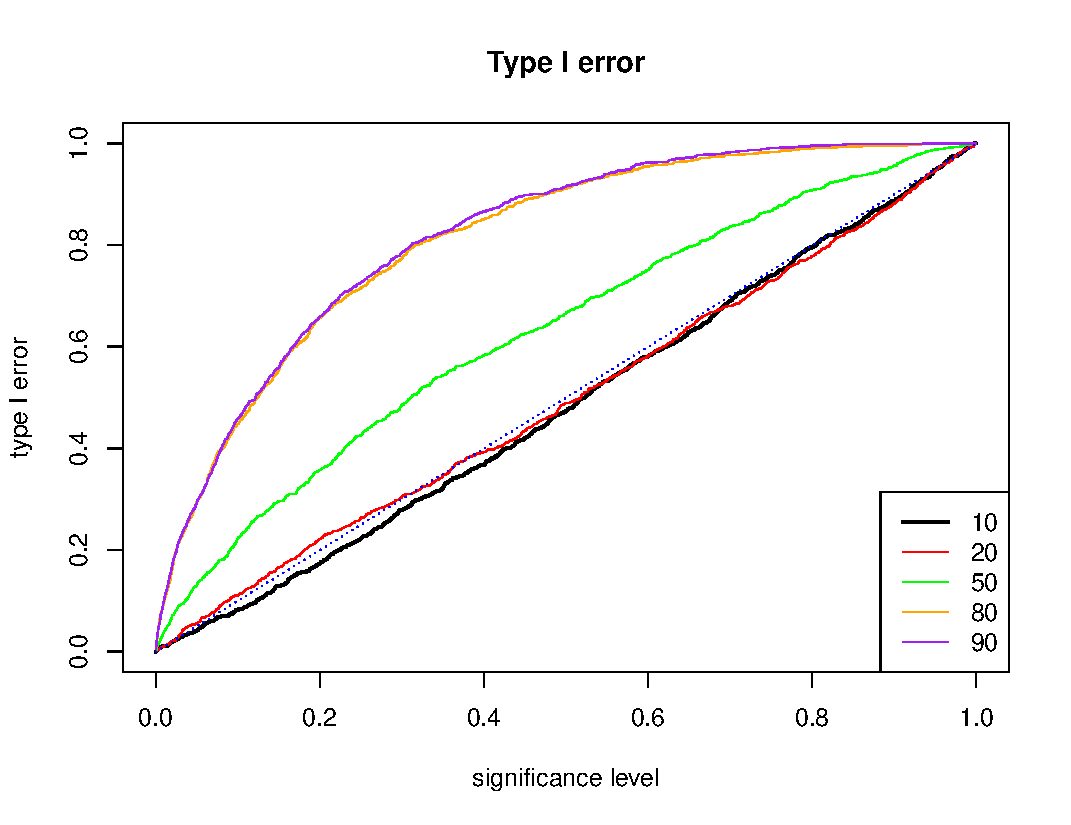
\includegraphics[width=\textwidth]{type1error_sum_ev.pdf}
			\caption{Ошибка первого рода (Sum).}
		\end{subfigure}\hspace{\fill}
		\begin{subfigure}[t]{0.45\textwidth}
			\centering
			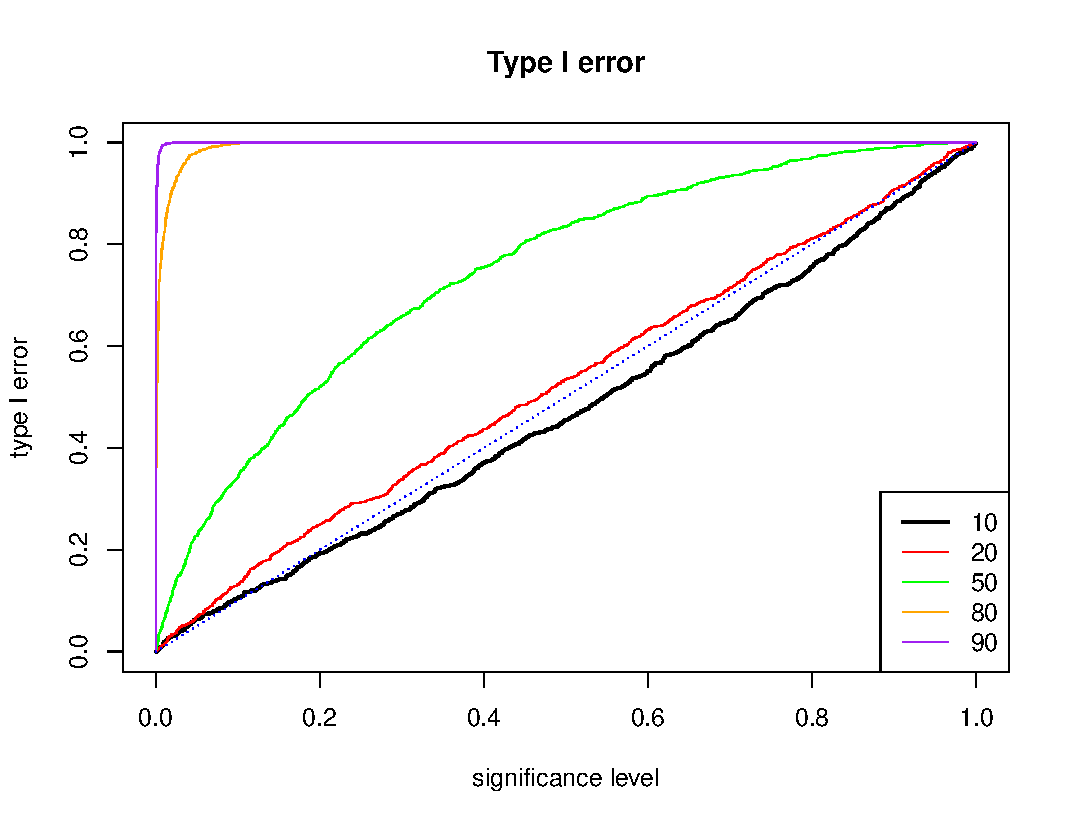
\includegraphics[width=\textwidth]{type1error_mssa_ev.pdf}
			\caption{Ошибка первого рода (базовый MSSA).}
		\end{subfigure}
		\bigskip
		\begin{subfigure}[t]{0.45\textwidth}
			\centering
			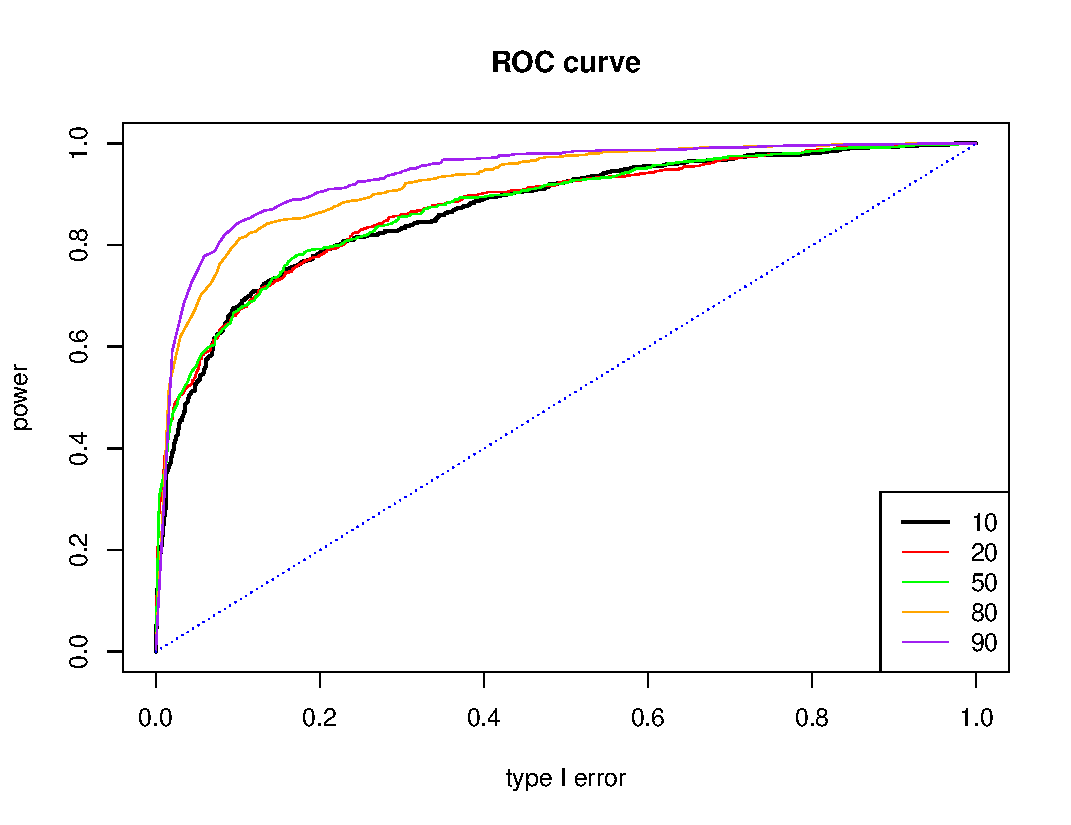
\includegraphics[width=\textwidth]{roc_sum_ev.pdf}
			\caption{ROC-кривая (Sum).}
		\end{subfigure}\hspace{\fill}
		\begin{subfigure}[t]{0.45\textwidth}
			\centering
			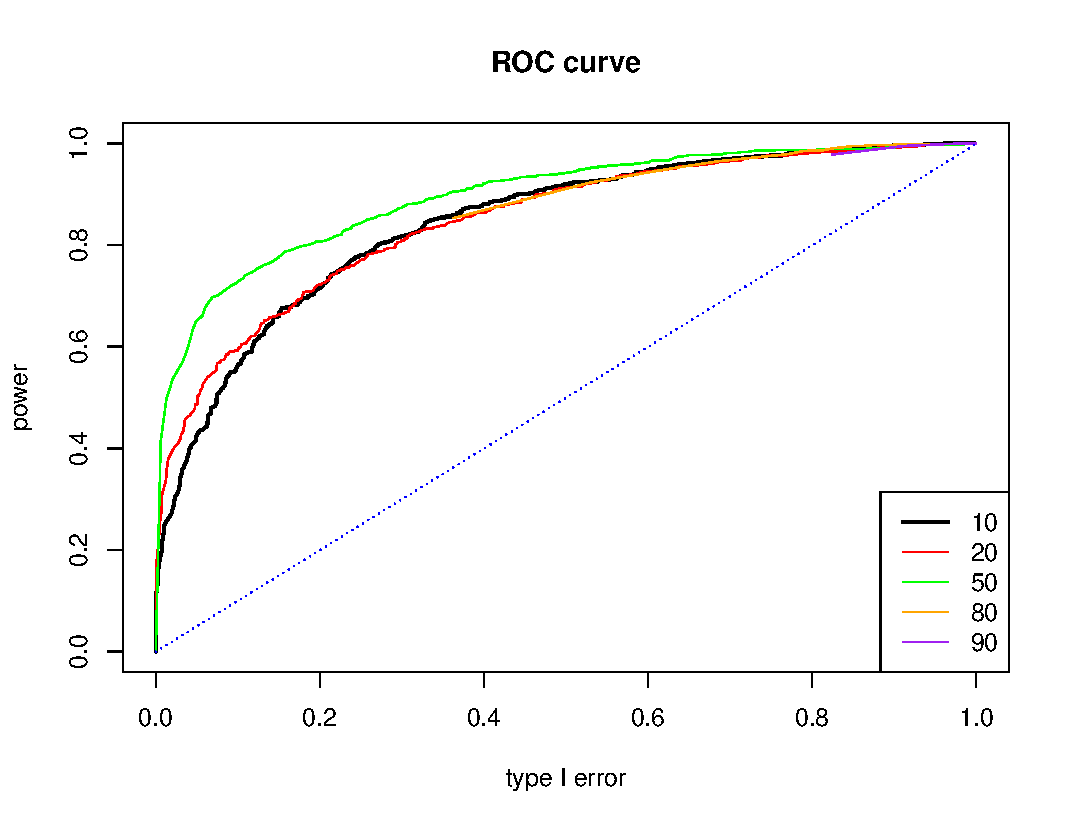
\includegraphics[width=\textwidth]{roc_mssa_ev.pdf}
			\caption{ROC-кривая (базовый MSSA).}
		\end{subfigure}
		\caption{Сравнение методов Sum и базового MSSA (проекция на собственные векторы).}
		\label{fig:sum_ev}\textsc{}
	\end{figure}
	\begin{figure}
		\captionsetup[subfigure]{justification=Centering}
		\begin{subfigure}[t]{0.45\textwidth}
			\centering
			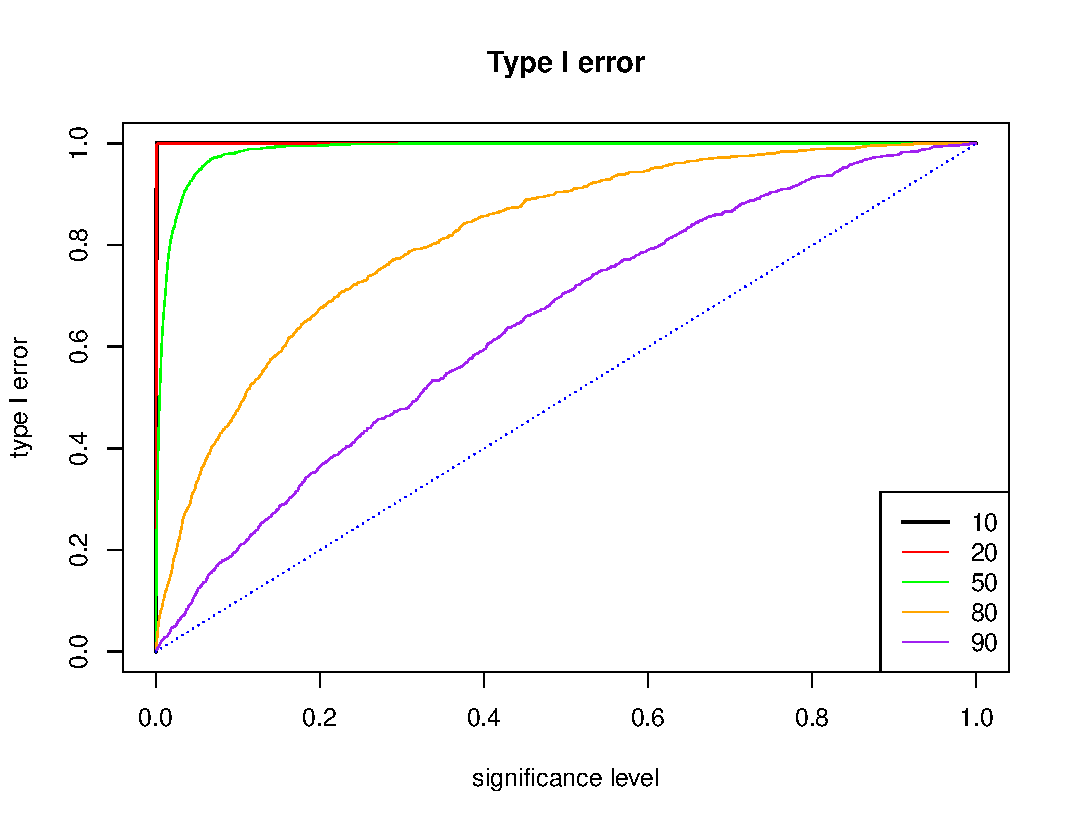
\includegraphics[width=\textwidth]{type1error_sum_fa.pdf}
			\caption{Ошибка первого рода (Sum).}
		\end{subfigure}\hspace{\fill}
		\begin{subfigure}[t]{0.45\textwidth}
			\centering
			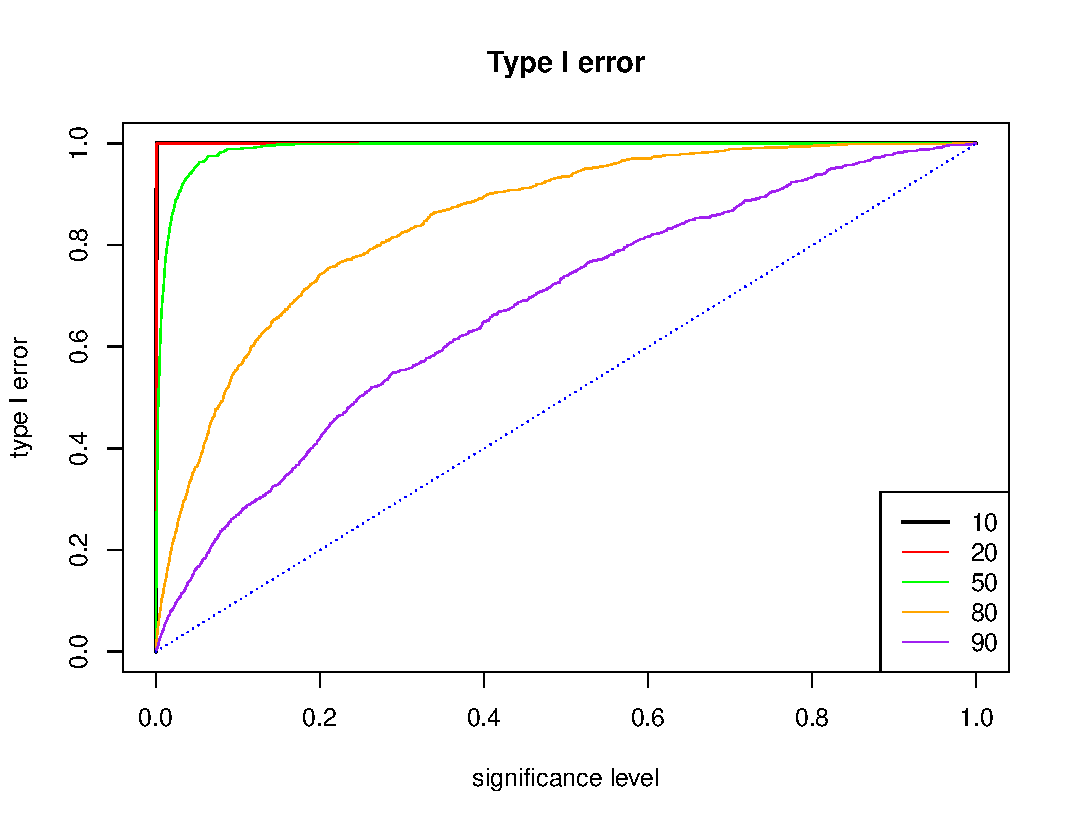
\includegraphics[width=\textwidth]{type1error_mssa_fa.pdf}
			\caption{Ошибка первого рода (базовый MSSA).}
		\end{subfigure}
		\bigskip
		\begin{subfigure}[t]{0.45\textwidth}
			\centering
			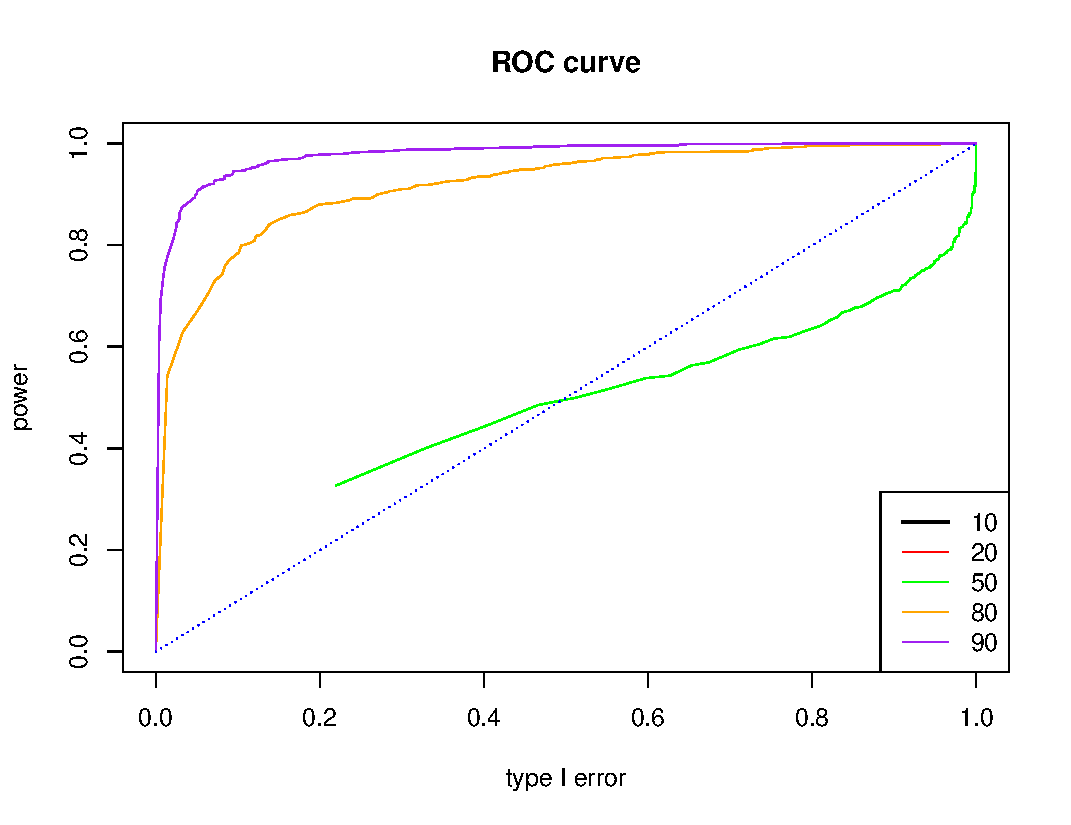
\includegraphics[width=\textwidth]{roc_sum_fa.pdf}
			\caption{ROC-кривая (Sum).}
		\end{subfigure}\hspace{\fill}
		\begin{subfigure}[t]{0.45\textwidth}
			\centering
			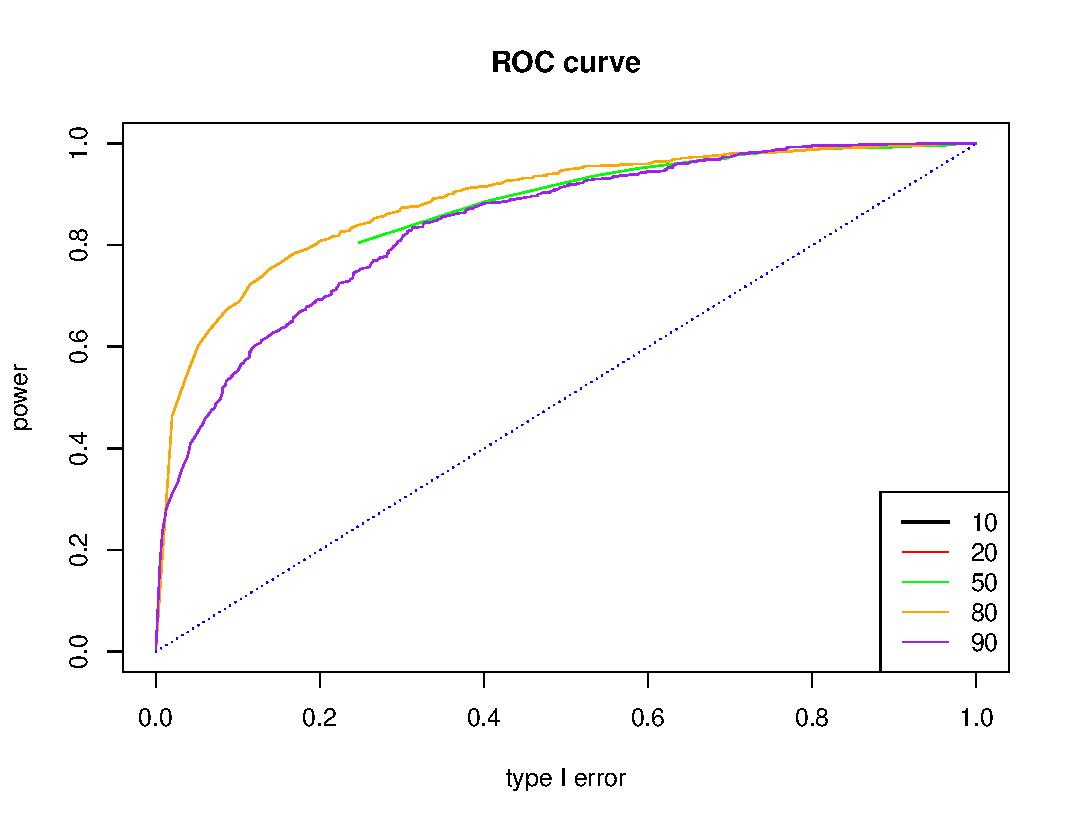
\includegraphics[width=\textwidth]{roc_mssa_fa.pdf}
			\caption{ROC-кривая (базовый MSSA).}
		\end{subfigure}
		\caption{Сравнение методов Sum и базового MSSA (проекция на факторные векторы).}
		\label{fig:sum_fa}
	\end{figure}
		\begin{figure}
		\captionsetup[subfigure]{justification=Centering}
		\begin{subfigure}[t]{0.45\textwidth}
			\centering
			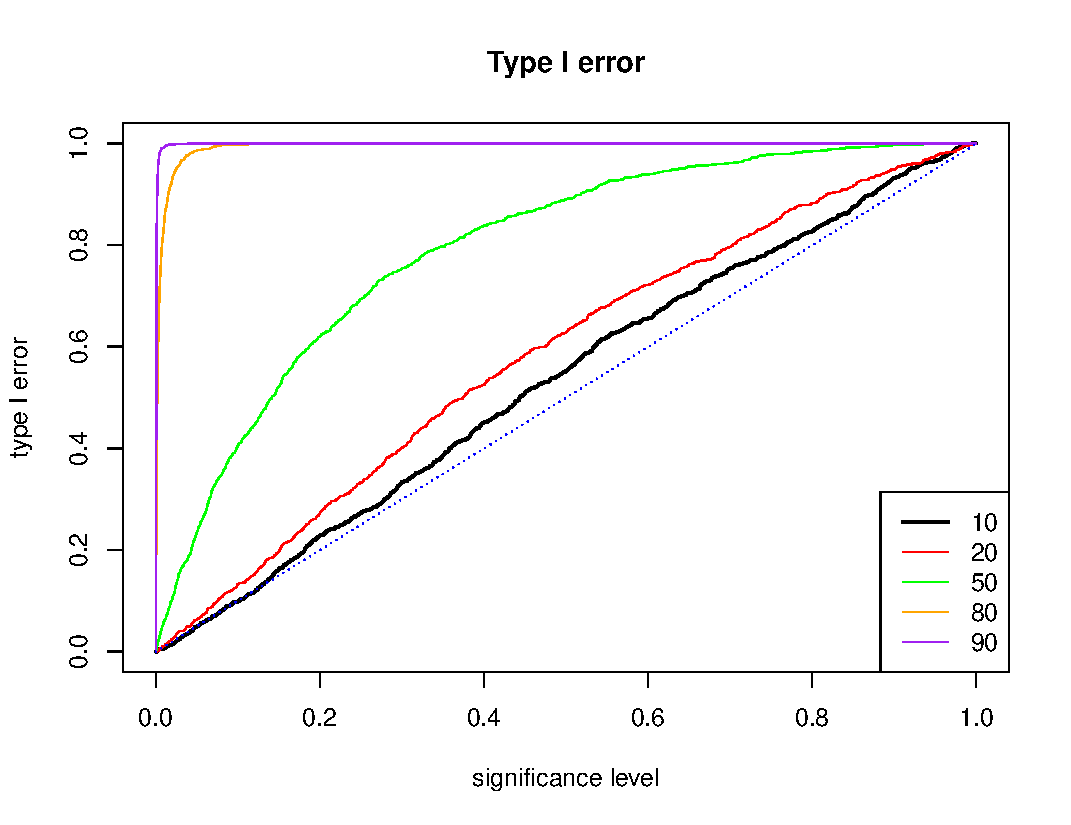
\includegraphics[width=\textwidth]{type1error_block_ev.pdf}
			\caption{Ошибка первого рода (Block).}
		\end{subfigure}\hspace{\fill}
		\begin{subfigure}[t]{0.45\textwidth}
			\centering
			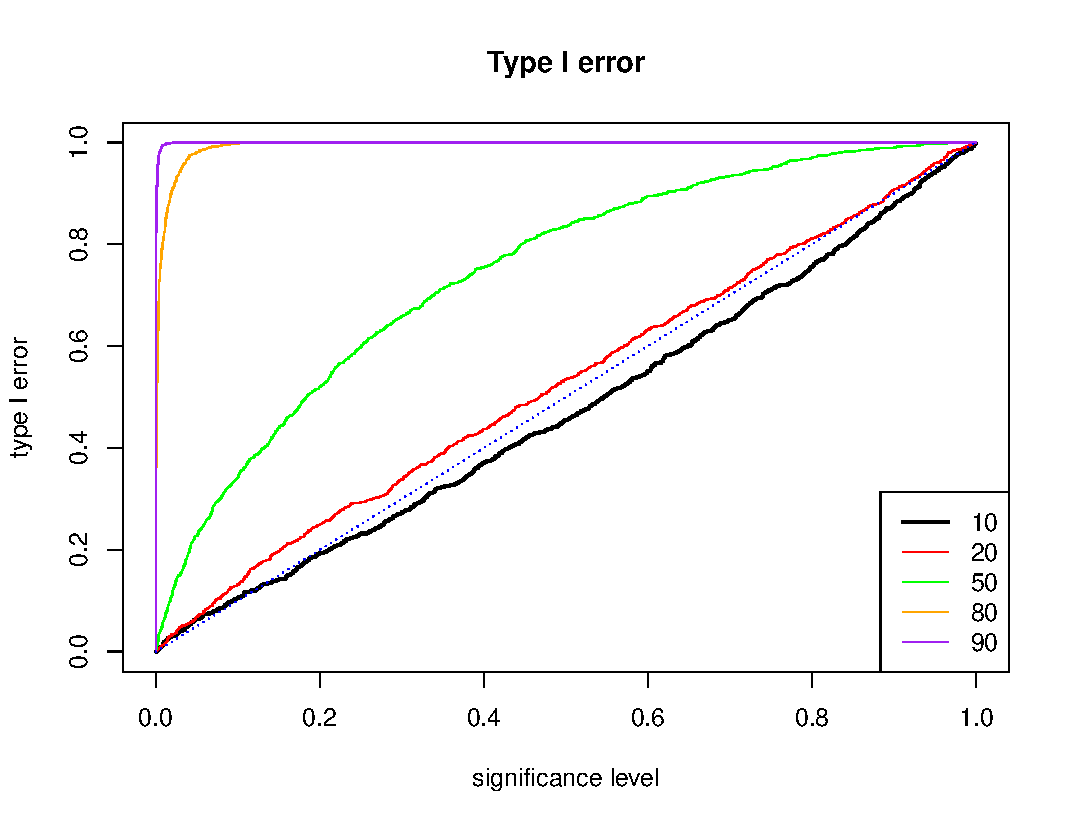
\includegraphics[width=\textwidth]{type1error_mssa_ev.pdf}
			\caption{Ошибка первого рода (базовый MSSA).}
		\end{subfigure}
		\bigskip
		\begin{subfigure}[t]{0.45\textwidth}
			\centering
			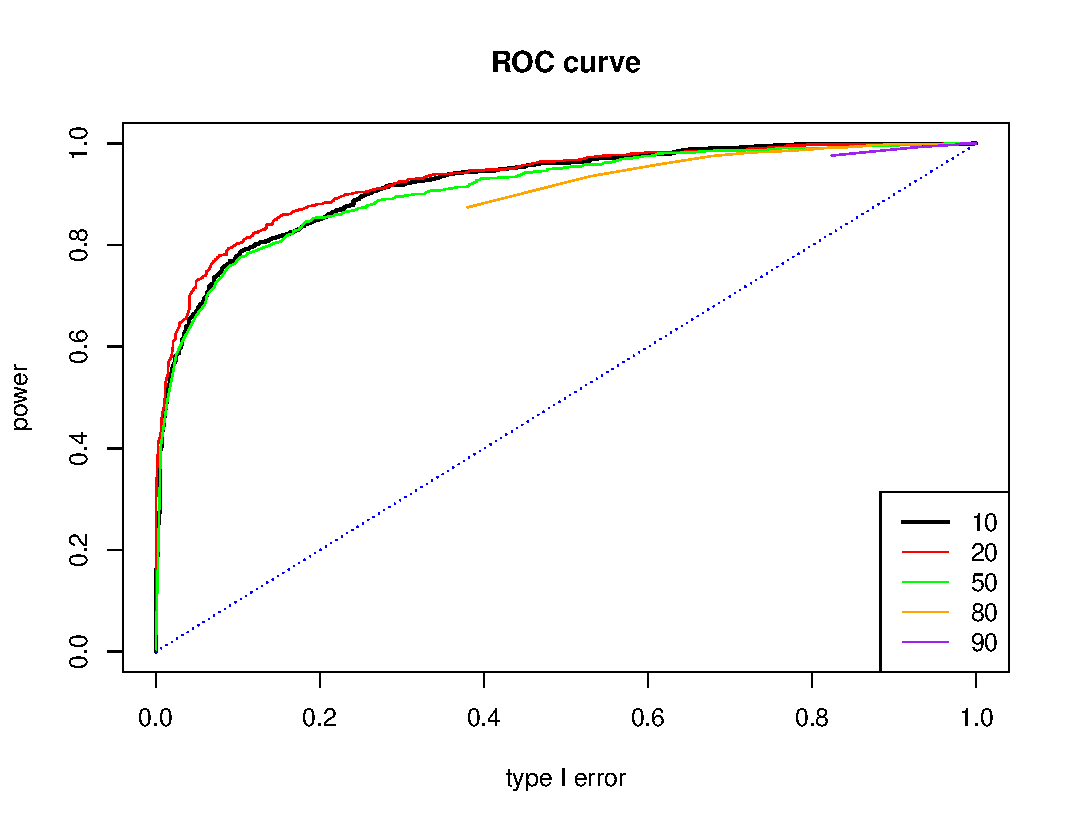
\includegraphics[width=\textwidth]{roc_block_ev.pdf}
			\caption{ROC-кривая (Block).}
		\end{subfigure}\hspace{\fill}
		\begin{subfigure}[t]{0.45\textwidth}
			\centering
			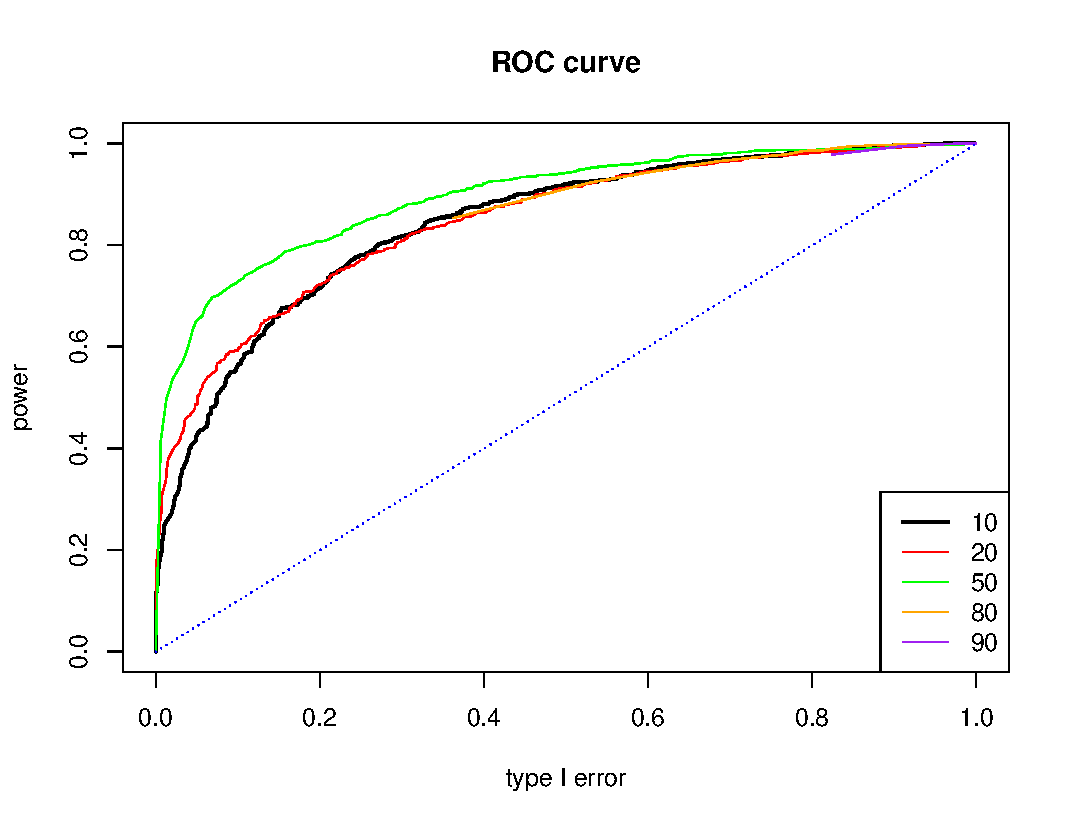
\includegraphics[width=\textwidth]{roc_mssa_ev.pdf}
			\caption{ROC-кривая (базовый MSSA).}
		\end{subfigure}
		\caption{Сравнение методов Block и базового MSSA (проекция на собственные векторы).}
		\label{fig:block_ev}
	\end{figure}
		\begin{figure}
		\captionsetup[subfigure]{justification=Centering}
		\begin{subfigure}[t]{0.45\textwidth}
			\centering
			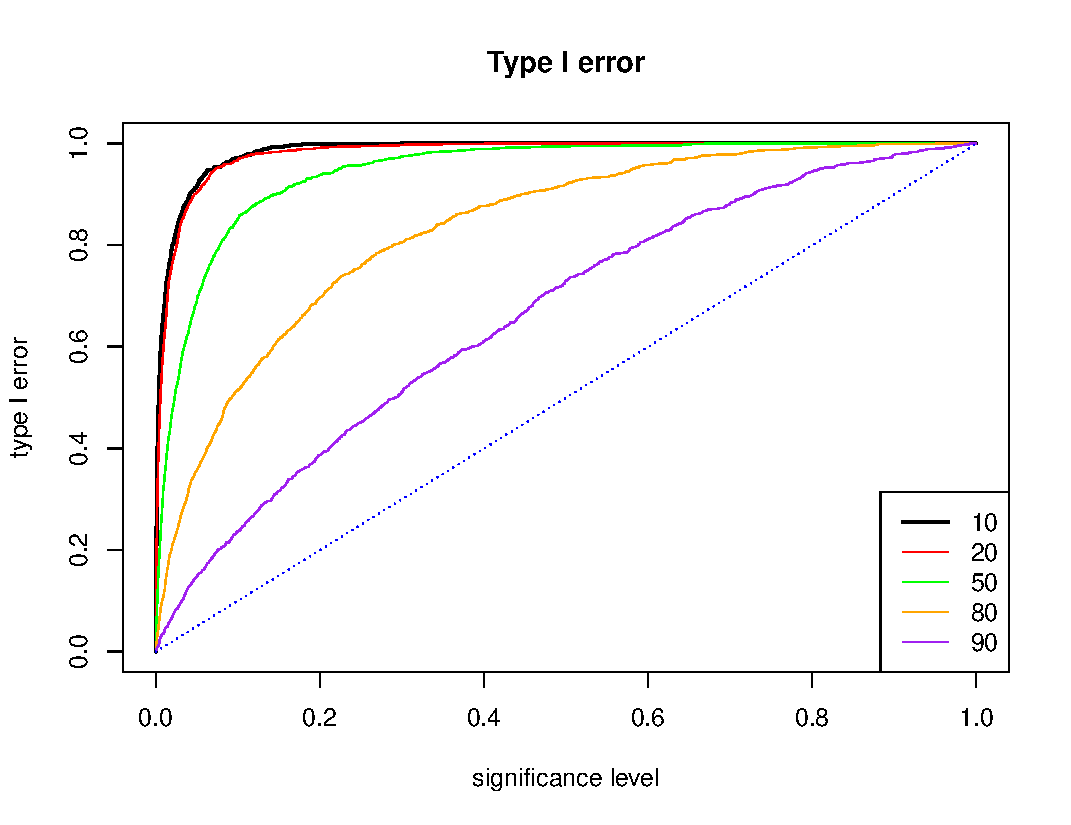
\includegraphics[width=\textwidth]{type1error_block_fa.pdf}
			\caption{Ошибка первого рода (Block).}
		\end{subfigure}\hspace{\fill}
		\begin{subfigure}[t]{0.45\textwidth}
			\centering
			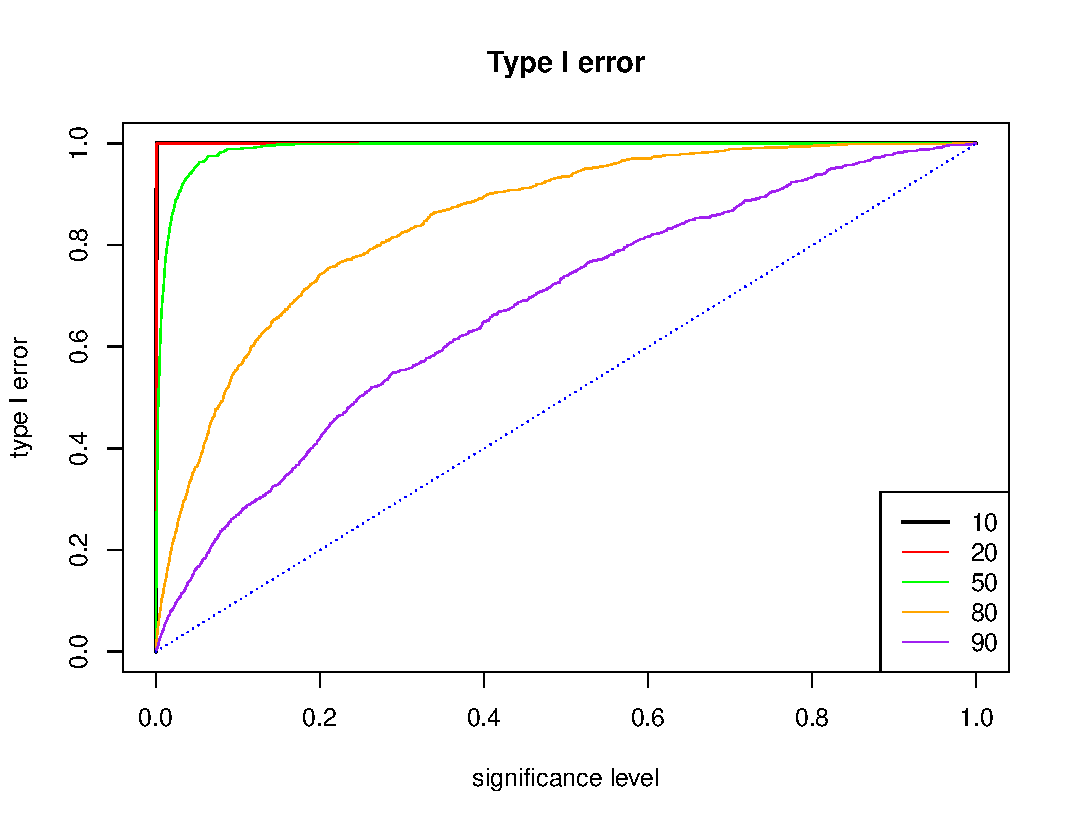
\includegraphics[width=\textwidth]{type1error_mssa_fa.pdf}
			\caption{Ошибка первого рода (базовый MSSA).}
		\end{subfigure}
		\bigskip
		\begin{subfigure}[t]{0.45\textwidth}
			\centering
			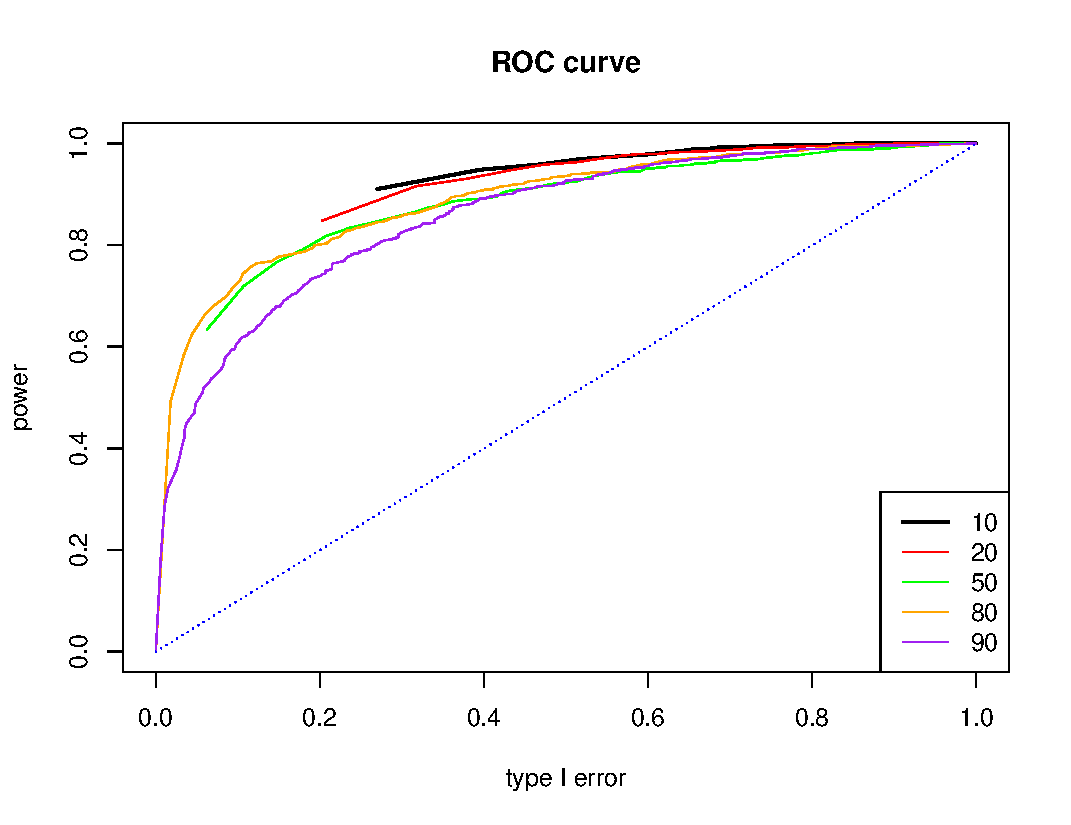
\includegraphics[width=\textwidth]{roc_block_fa.pdf}
			\caption{ROC-кривая (Block).}
		\end{subfigure}\hspace{\fill}
		\begin{subfigure}[t]{0.45\textwidth}
			\centering
			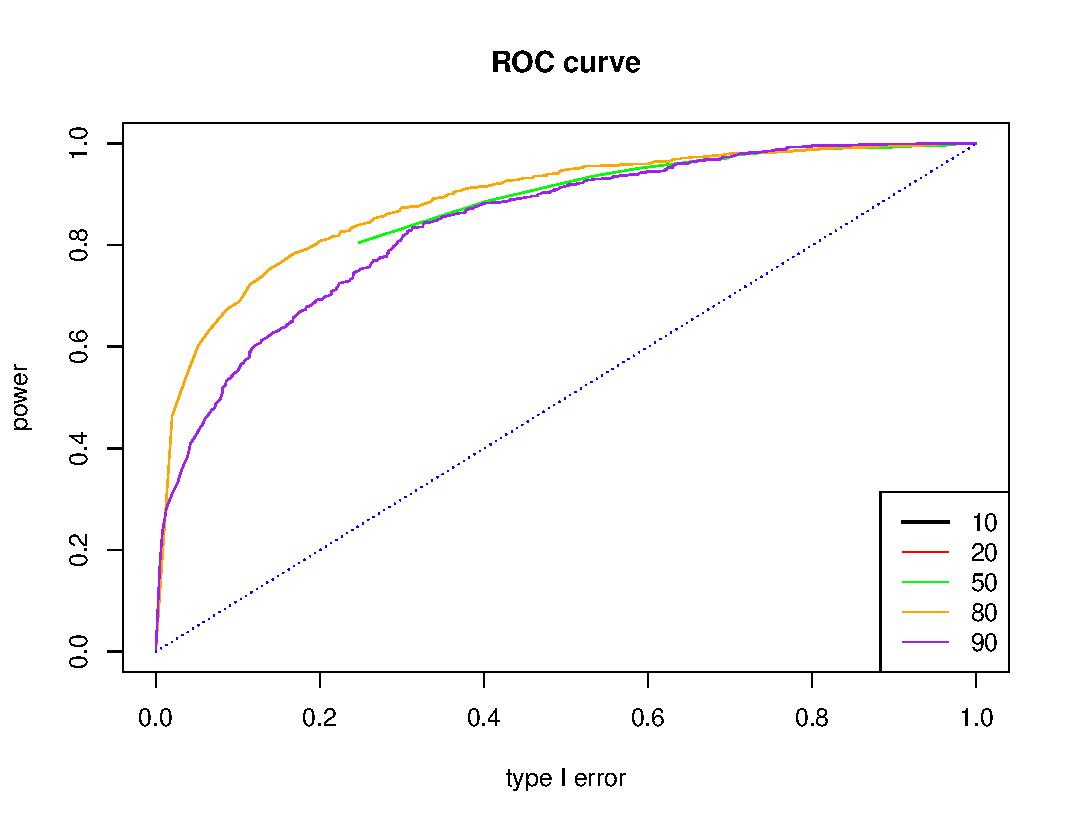
\includegraphics[width=\textwidth]{roc_mssa_fa.pdf}
			\caption{ROC-кривая (Block).}
		\end{subfigure}
		\caption{Сравнение методов Block и базового MSSA (проекция на факторные векторы).}
		\label{fig:block_fa}
	\end{figure}
	\conclusion
	TODO
	\bibliographystyle{ugost2008}
	\bibliography{report}
\end{document}